 



\section{Empirical Study}

\begin{figure*}[ht]
	\centering
	%[trim=left bottom right top, clip]
	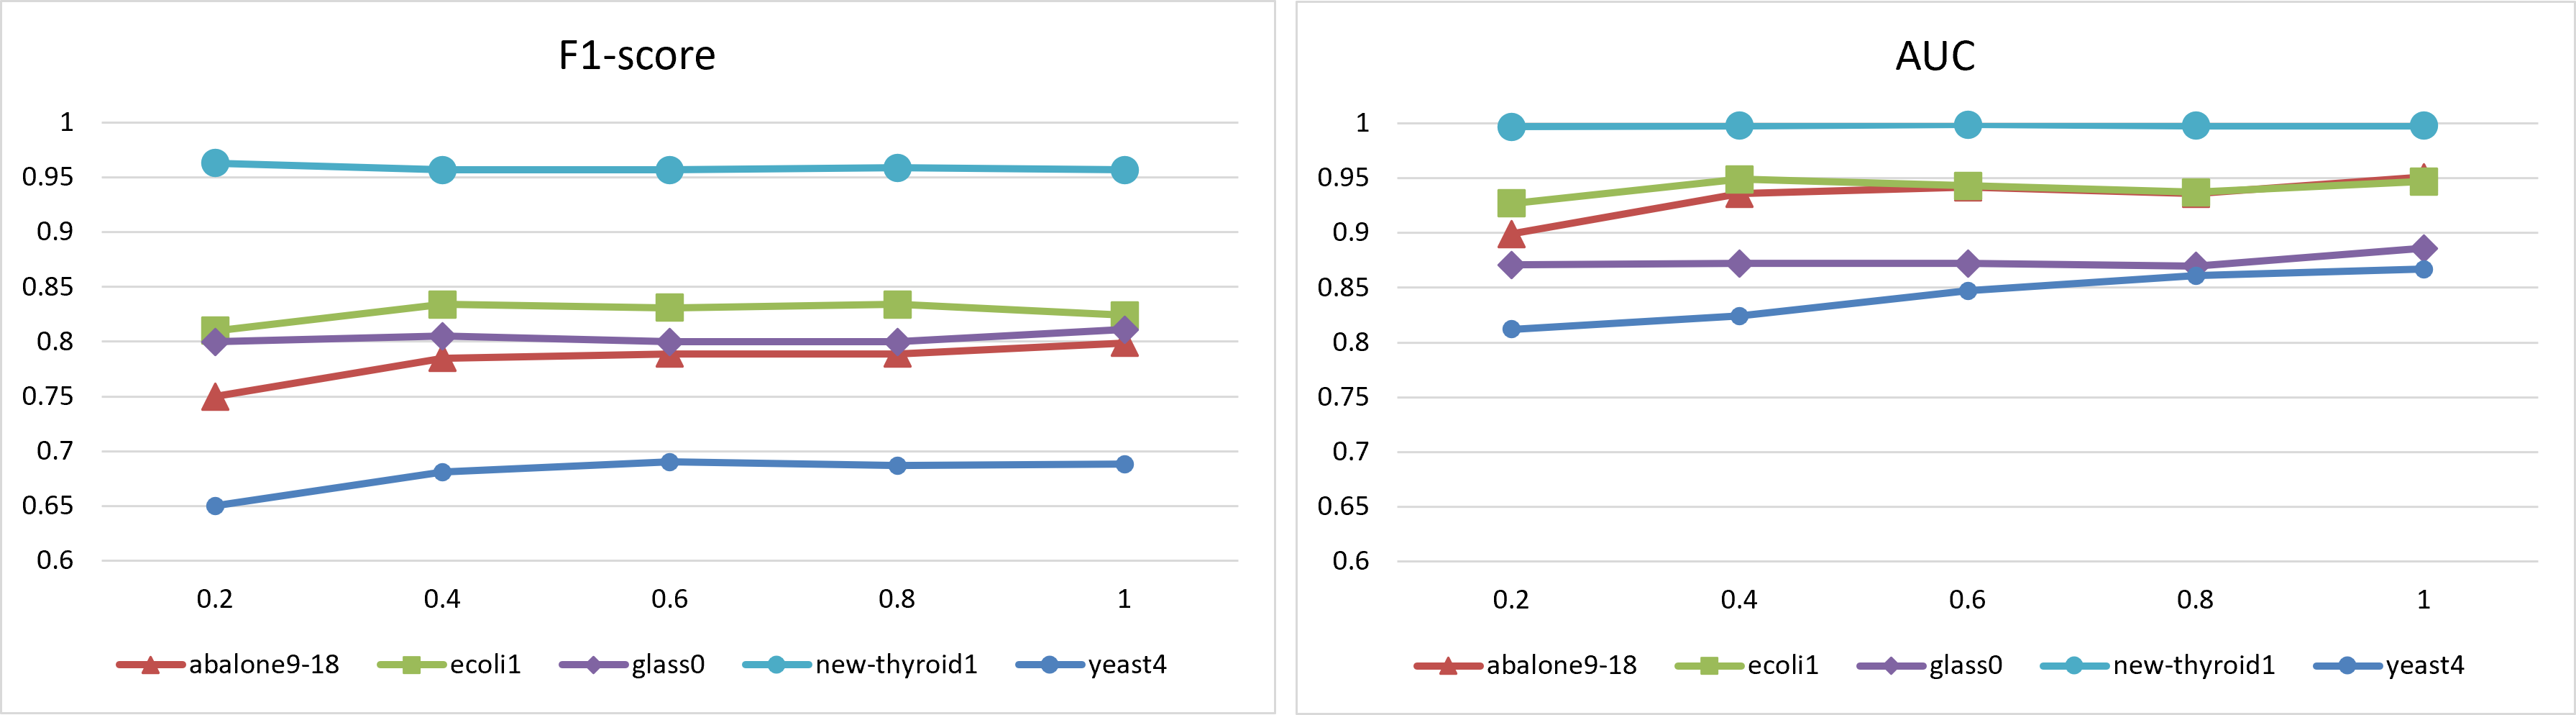
\includegraphics[width=0.98\linewidth, trim=5 10 10 10, clip ]{Figures/r_impact}
	\caption{F1-score and AUC results with varying Gaussian standard deviation (ranging from 0.2R to R).}
	\label{fig:r_result}
\end{figure*}

\begin{figure*}[h]
	\centering
	%[trim=left bottom right top, clip]
	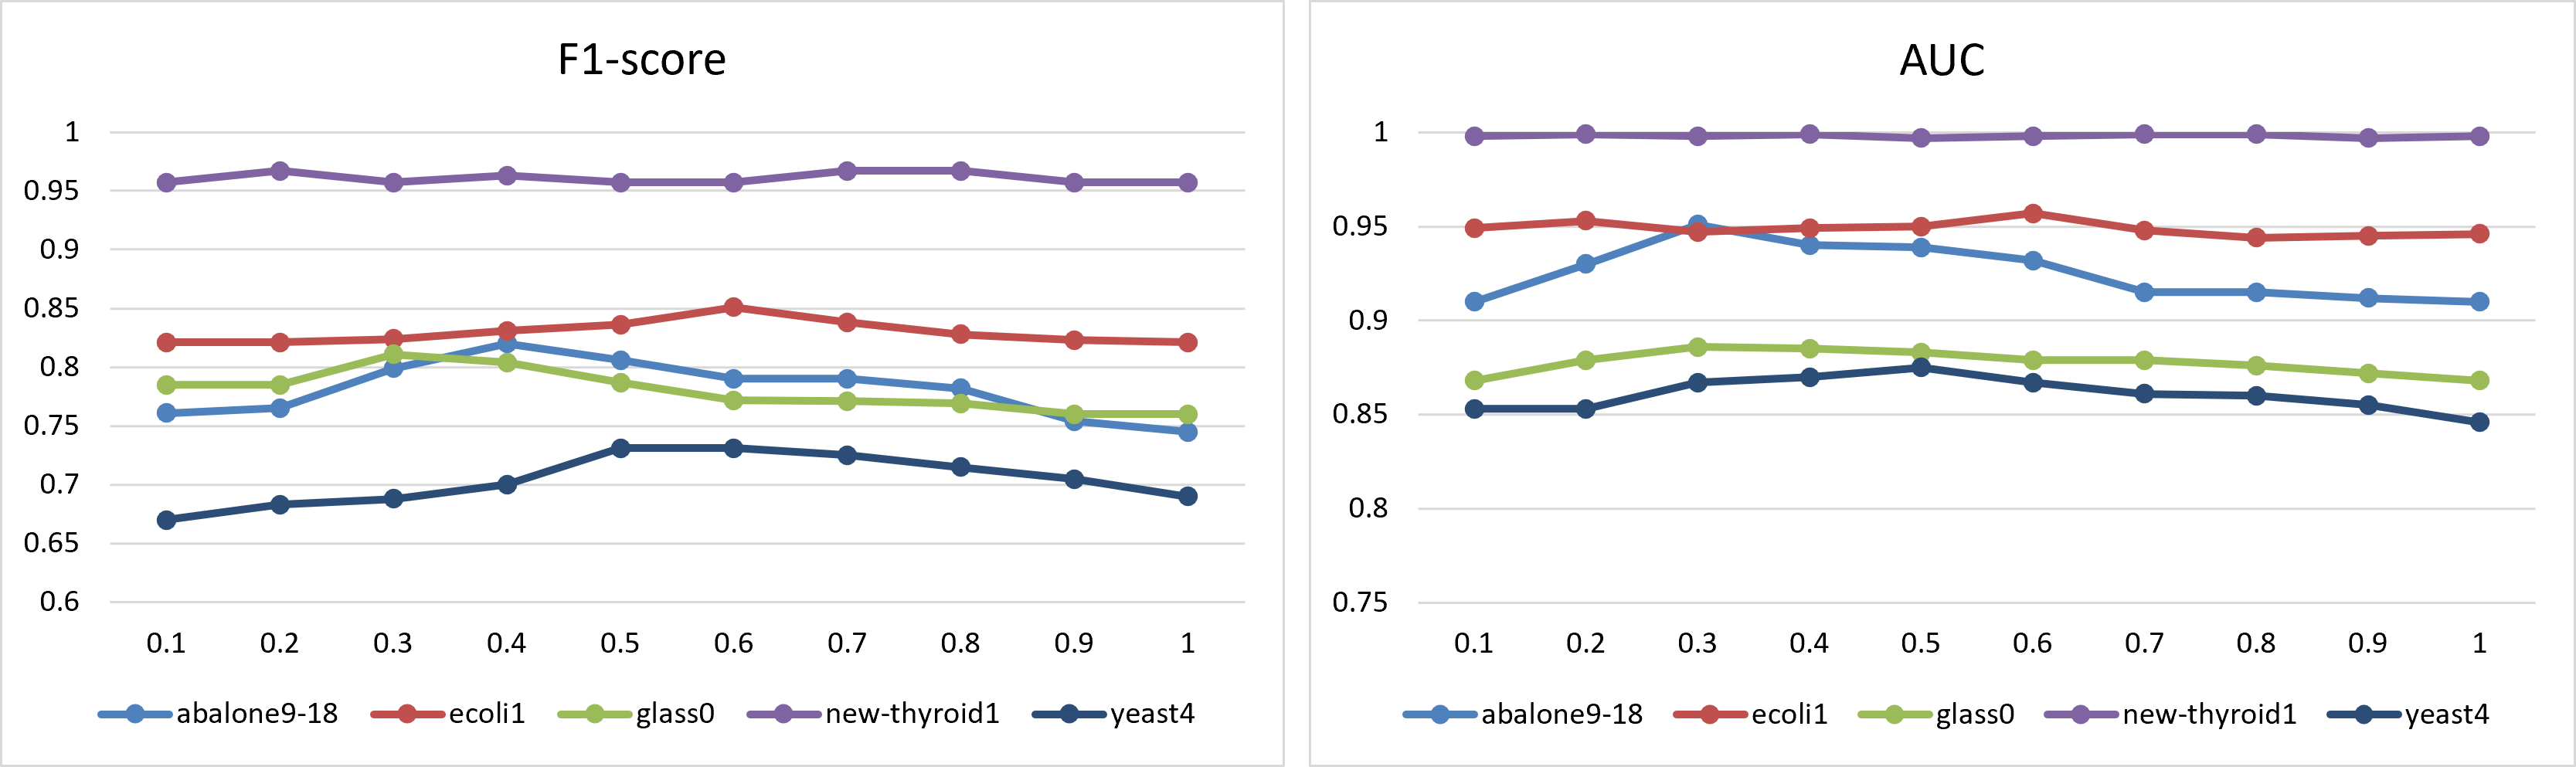
\includegraphics[width=0.98\linewidth, trim=5 10 10 10, clip ]{Figures/threshold_impact}
	\caption{F1-score and AUC results with varying informative portion IP.}
	\label{fig:ip_result}
\end{figure*}

\subsection{Empirical study on the impact of radius factor r.}
\label{sec:simpor_r_distribution_impact}
In this section, we study how the classification performance is impacted by different generation radius factor $r$ in Equation \ref{equ:r_dist}. The classification performance is measured under different distribution settings of the radius r as it controls how far synthetic data are generated from its original minority sample. We use different parameters for the Gaussian distribution $\mathcal{N}(\mu ,\,{(\alpha R)}^{2})$. Particularly, we fix the mean value to zero and change $\alpha$ from 0.2 to 1 with steps of 0.2 so that the Gaussian standard deviation $\alpha R$ will range from 0.2R to R. To save space, we arbitrarily select 5 datasets to conduct this experiment. The classification results are shown in Figure \ref{fig:r_result}. 


The figure obtained from the experiment indicates that the r factor, with a radius distribution standard deviation ranging from 0.6R to R, has minimal impact on the classification performance. While there are slight variations within the $\alpha$ range of 0.6 to 1, the performance improves between 0.2 to 0.6 (such as for ecoli1, abalone9-18, and yeast4). This is because the performance mainly depends on the classifier's decision boundary, and the synthetic data are placed far away from the decision boundary towards the minority class area; thus,  the radius does not have much effect on the accuracy results. However, in the case of multi-classed data, the performance might be affected by a significant value of R. 

\subsection{Empirical study on the impact of informative portion (IP).}
This section studies the empirical impact of the informative portion (IP) in Section \ref{sec:EAL}. This portion works as a threshold to adjust how many samples are taken into consideration of informative samples. To save space, we study five datasets used in Section \ref{sec:simpor_r_distribution_impact}. Different values of IP ranging from 0.1 to 1 are applied, and the classification performance results are shown in Figure \ref{fig:ip_result}.


As we can see from the figure, while datasets with outstanding performance (new-thyroid1, ecoli1) have little impact, there are fluctuations in other datasets' F1-score and AUC score  (abalonce9-18, glass0, yeast4). This is because, for the easy-separated dataset such as new-thyroid1 and ecoli1, the IP change does not affect the classification performance as the data classes are easily separated. While in more challenging datasets, IP changes might affect the balance at the informative region; thus, this leads to performance variations. The resulting figure also suggests tuning IP for each dataset between a range of (0.2, 0.6) could achieve higher performance.



